\documentclass[10pt]{article}\usepackage[margin=.55in]{geometry}\usepackage[T1]{fontenc}\usepackage{graphicx}\setlength{\parindent}{0pt}\setlength{\parskip}{5pt}\sloppy\begin{document}{\large Private qualifier descriptor release transport}\par Task T-1479. 3 November 2026.\par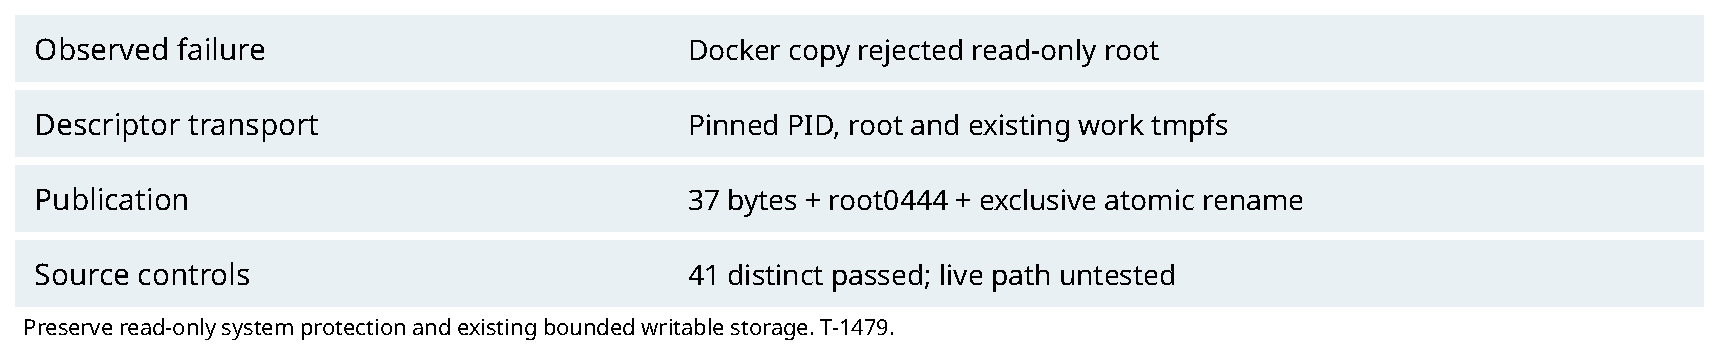
\includegraphics[width=\linewidth]{diagram.pdf}\par The source successor replaces Docker archive copy with descriptor-relative publication into the existing work tmpfs. The first authorized120-second/2GiB wrapper passed39 tests in0.403639 seconds. After independent review corrections, the separately authorized second wrapper passed52 executions (41 distinct controls and11 inherited duplicates) in0.212249 seconds; unittest reports0.060 seconds. Both attempts and the original tested source are retained. Inputs remained unchanged and the child was reaped. Gate source6548 is byte-identical. Corrected source awaits independent review; no runtime admission is asserted.

Observed trigger. Qualification-v4 passed Q0, then failed Q1 release with container rootfs is marked read-only. Existing gate readiness and host ancestry were observed before copy failed. This packet preserves that failure and all predecessor sources. No retry, proc write, Docker, systemd, mount, container or cloud action occurred here.

Construction. The existing private contract now opens held proc/PID and pidfd anchors, verifies PID start ticks and cgroup against the independently inspected container, and follows only the kernel root magic link. Ordinary work and token components are descriptor-relative and nofollow. Actual work FD must be root-owned mode1777 tmpfs, writable with nosuid/nodev/noexec and at most16MiB; the root FD must remain read-only. Current ancestry, deadlines and pending signals are rechecked before publication.

Publication. An exclusively created nonce staging file receives exactly37 bytes, explicit root0444 metadata, fsync and descriptor readback. A sole renameat2 NOREPLACE publishes the completed file. Existing final files of every type cannot be replaced. Separate exclusively created host receipt files, each file and parent-directory synced, retain possible release before publication; the full boundary callback runs again after this I/O; interruption after the attempt never triggers retry or final-token rollback. Cleanup removes only an inode-matched staging file before publication; exact container cleanup remains with the enclosing supervisor. Existing case results still require all logs, expected exits and strict diff checks.

Controls. Preserved22 tests include an adapted AST release-order check;17 initial new controls cover real unprivileged temporary-file rename, UMask0077, short/zero writes, collisions, token bytes/mode/link count, invalid nonce, cleanup substitution and uncertain completed rename. Root UID/GID alone are substituted for these local tests. Mocked kernel controls cover PID lifetime, proc access, ancestry, final revalidation, work custody/filesystem flags and FD closure. No local test establishes actual proc-root ptrace permission or container mount behavior.

Source design. The exact preceding design is ../runtime-private-gate-release-fd/DESIGN.md, SHA ed60668b4c86e4e7970b0d756968e4475a6b4db0719453ed4953cda0e2079f6b. It records primary Linux proc, pidfd, open, renameat2, statfs and Python os documentation. A typed Linux x86-64 libc adapter fails closed on unavailable ABI or symbols. The four-file qualifier source closure remains intact; only supervise and private contract production files change. Draft admission remains false.

Boundary. Held descriptors prevent PID reuse redirecting publication; they do not keep a process alive or make all observations atomic. Same-work inference uses the trusted gate, fixed mounts and PID1 single-process controls; gate readiness binds cgroup identity rather than work inode. Permission denial causes retained failure without capability expansion. Independent source review and a separately admitted qualification must establish the live integration path.


Review corrections and procedural error. Independent review found that overwriting transport.json could destroy the sole durable possible-release record and that receipt I/O could defer a signal beyond the final check. Both are corrected and two targeted controls check boundary denial during recording and prepublication-record survival when confirmation fails. The second standalone freeze-generation command failed because its path was relative to the repository while cwd was already the packet. The shell continued into the runner, which wrote attempt2/inputs.json before launching tests and verified unchanged inputs afterward. AMENDMENT.md already froze the additional allowance. This error and52 executions including11 inherited duplicates are preserved; no test retry followed. Total observed test-wrapper time is0.615888 seconds against240 seconds authorized ceilings.
\end{document}